\documentclass[journal]{IEEEtran}
\usepackage{verbatim}
\usepackage{cite}
% The latest version can be obtained at:
% http://www.ctan.org/tex-archive/macros/latex/contrib/cite/

% *** GRAPHICS RELATED PACKAGES ***
%
\ifCLASSINFOpdf
   \usepackage[pdftex]{graphicx}
  % declare the path(s) where your graphic files are
   \graphicspath{{./figures/png/}}
  % and their extensions so you won't have to specify these with
  % every instance of \includegraphics
   \DeclareGraphicsExtensions{.pdf,.jpeg,.png}
\fi
\usepackage[cmex10]{amsmath}
% *** SPECIALIZED LIST PACKAGES ***
%
%\usepackage{algorithmic}
% http://www.ctan.org/tex-archive/macros/latex/contrib/algorithms/
% http://algorithms.berlios.de/index.html
% http://www.ctan.org/tex-archive/macros/latex/contrib/algorithmicx/

% *** ALIGNMENT PACKAGES ***
%
\usepackage{array}
% http://www.ctan.org/tex-archive/macros/latex/required/tools/

\usepackage{mdwmath}
\usepackage{mdwtab}

\hyphenation{op-tical net-works semi-conduc-tor}

\begin{document}
\title{Instrumentation For The Anodization and Characterization of Titanium Electrodes for Electrolytic Capacitors}

\author{M. DeLibero,~\IEEEmembership{Student Member,~IEEE,}
        S. Ehret,~\IEEEmembership{Member,~IEEE,}
        and F. Merat,~\IEEEmembership{Senior Member,~IEEE}%

\thanks{This work was supported by ARPA-E under grant \#DE-AR0000116.}}

\maketitle

\begin{abstract}
This paper presents a custom circuit for controlling the anodization of titanium capacitors and characterizing their performance. The circuitry provides a constant current source of 0-100mA up to a compliance voltage of 30V. The system can monitor and record leakage currents down to 10 nA over periods of up to 24 hours. Typical results obtained using sputtered titanium-zirconium capacitors are presented.
\end{abstract}

\begin{IEEEkeywords}
Capacitor, Switched Capacitor Circuits
\end{IEEEkeywords}

\IEEEpeerreviewmaketitle

\section{Introduction}

\IEEEPARstart{C}{apacitors} with high energy and power are essential for efficient management of electrical power.  Order of magnitude increases are desired for energy and power density. This may be possible with new self-repairing titanate dielectric capacitors using high surface area doped titanium and doped zirconium-titanium.  Anodizing at DC voltages forms a uniform dielectric film of doped titanium (the energy density of this dielectric is estimated to be on the order of 150J/$cm^3$) \cite{tiSponge}. This and the volume fraction of dielectric determines the energy density of the capacitor.

One of the major problems plaguing titanium electrolytic capacitors has been their high leakage currents \cite{tiCharHag}. In order to further research into titanium capacitors, custom anodization instrumentation has been developed to anodize and characterize a large number of candidate titanium capacitor materials. This instrumentation was necessary because conventional systems do not have the necessary dynamic range (1A-1nA measurement) or repeatability needed in this application.


\subsection{Anodization Process and Requirements}

Anodization is the act of growing an oxide layer (dielectric) on top of a metal anode. Dielectrics are benificial because they allow capacitors to store more energy for a given electric field \cite{cwruEncDie}. The anodization process is preformed by connecting a voltage or current source to an anode and a cathode and immersing them in an electrolyte solution as shown in Fig. ~\ref{fig:anodSetup}

\begin{figure}[here]
\centering
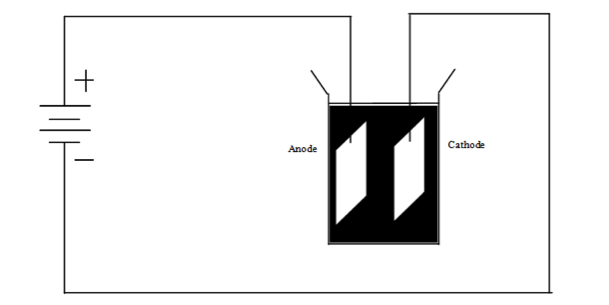
\includegraphics{anodSetup}
\caption{Anodization Setup}
\label{fig:anodSetup}
\end{figure}


Referring to Fig. ~\ref{fig:anodSetup}, in the simplest case, the current transfer is an ionic transfer where the Ti anode reacts with $O_{2}$ to create a $TiO_{2}$ oxide layer. The reaction at the metal-oxide surface can be written as:

\begin{equation}
Ti + 0_2 => TiO_2 + 4e
\end{equation}
The titanium also reacts with the electrolyte solution to give off hydrogen:
\begin{equation}
Ti + 2H_20 => Ti0_2 + 4H+Ti0_2
\end{equation}
This hydrogen reacts with the electrons at the cathode to create hydrogen gas and complete the ionic circuit.
\begin{equation}
4H + 4e => 2H_20
\end{equation}

This process is very similar to anodizing aluminum. For an explanation of that process visit \cite{cwruEncAlanod}.

Since the rate of oxide formation is dependent on the charge transport into the anode during anodization \cite{tiMinit}, a current source was selected. A typical anodization process with a current source will see the current and voltage progress as in Fig. ~\ref{fig:anodCurve}.


\begin{figure}[here]
\centering
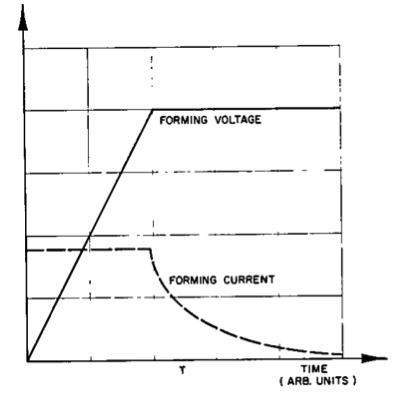
\includegraphics{anodCurve}
\caption{Anodization Curve \cite{tiMinit}}
\label{fig:anodCurve}
\end{figure}

Our typical anodization tests work with a constant current of 20mA and a forming voltage of 30V. The anodization reaches the forming voltage in periods on the order of 30 seconds. The forming voltage then remains constant while the leakage current decreases over  a much longer time period (on the order of 24 hours) to currents on the order of 1 uA or less. The exact times and values are dependent upon the material and the size of the electrode.

If a constant current is introduced, the voltage will (ideally) rise linearly with time. This will happen until the anode reaches the compliance voltage, at which point the current through the DUT will begin to drop off until it reaches the leakage current of the unpackaged capacitor. 

\section{Design and Implementation of Custom System Used for Anodization}

\begin{figure}[here]
\centering
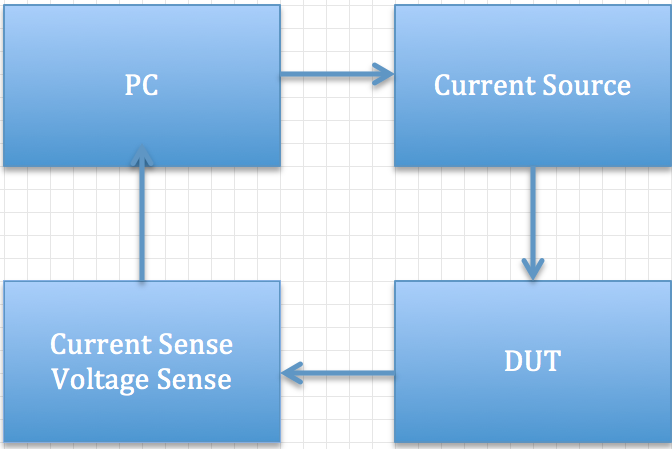
\includegraphics[width=3.5in]{blockDiagram}
\caption{Overall System Block Diagram}
\label{fig:blockDiagram}
\end{figure}

\subsection{Computer Control and Data Acquisition}

The user sets the test parameters of current, voltage compliance, and testing time. The anodization is then controlled by a set of Python scripts, which appropriately configure the hardware and control the data logging. Voltage and current measurements are sampled at a constant, high rate and all data is recorded. However, once the electrode has reached the forming voltage and the (leakage) current is slowly decreasing over time the data measurements are subsampled, and only a fraction of the sampled data is preserved.  (say more on this)

\subsection{Current Source}

An ideal current source has the ability to output a constant, DC, current to any load with infinite voltage compliance. This ability makes a current source an attractive tool to use in anodization due to its ability to tightly control the rate of oxide growth on the anode.

\begin{figure}[here]
\centering
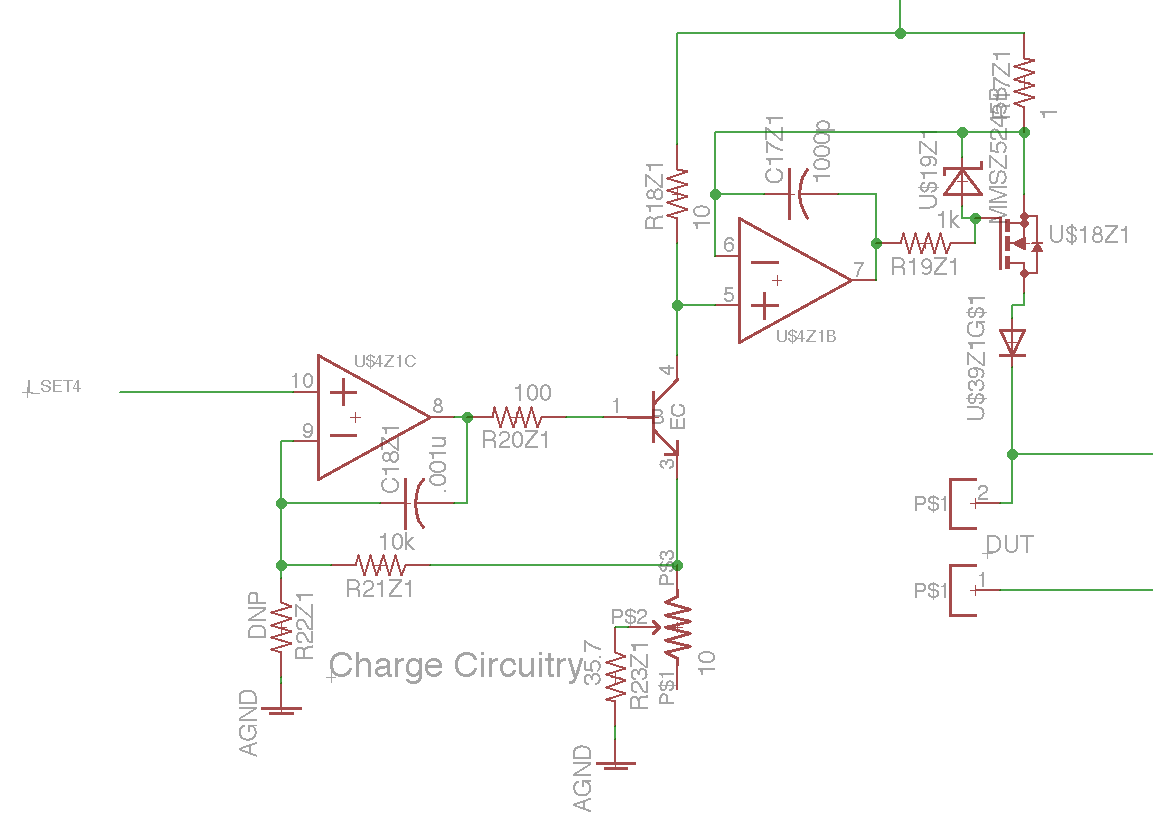
\includegraphics[width=3.5in]{currentMirror}
\caption{Current Control Circuitry}
\label{fig:currentMirror}
\end{figure}


The current source implementation (Fig. ~\ref{fig:currentMirror}) was chosen around an op-amp based current mirror. The op-amp on the left, U4Z1C, is used to set and regulate the current through R23. This current functions as the reference current on the left leg of the current mirror. The op-amp on the right, U4Z1B, forces the voltage drop across $R_{17}$ and $R_{18}$ to be the same, causing the current in the right leg to go as:

\begin{equation}
I_2 = I_1*R_{18}/R_{17}
\end{equation}

With the values chosen in this design, this equates to a 10x current amplification from the reference to the current output. The adjustable supply voltage is applied to the node connecting resistors $R_{17}$ and $R_{18}$. The current source will be able supply a constant current up to an effective compliance voltage of the supply voltage minus the voltage drops of $R_{17}$, the pass transistor, and the protection diode.

The real current source has several practical limitations that provide less than ideal performance. 

\begin{enumerate}
\item Pass transistor power rating
\item Digitization of current settings
\item Slight nonlinearity due to the pass diode
\end{enumerate}


\begin{figure}[here]
\centering
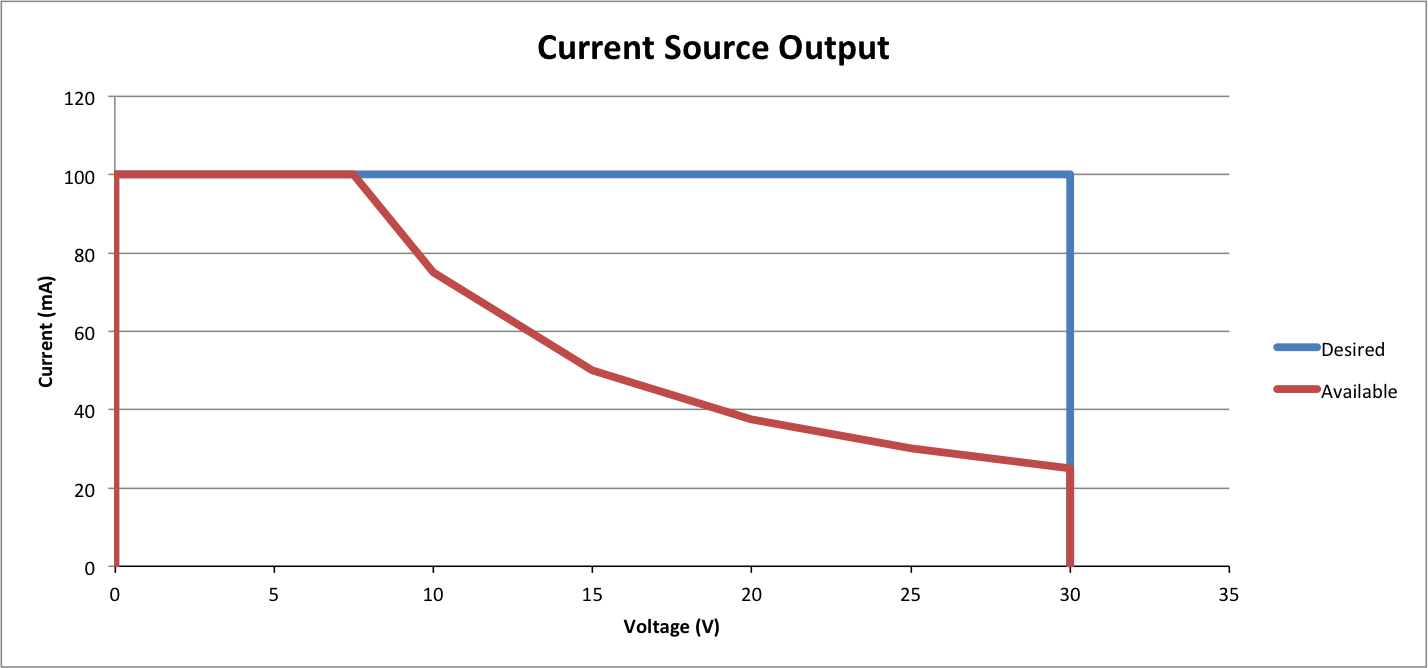
\includegraphics[width=3.5in]{safeOpArea}
\caption{Current Source: Safe Operating Area}
\label{fig:safeOpArea}
\end{figure}

The safe operating area (Fig.  ~\ref{fig:safeOpArea}) is smaller than the desired operating output of 30V at 100mA. This difference comes from the limitations in the power dissipation of the pass transistor, U18Z1, in Fig. ~\ref{fig:currentMirror}. Assuming the worse case scenario of a short on the output, the allowable output current for a given voltage compliance can be found as:

\begin{equation}
I_{out} = P_{rating} / V_{comp}
\end{equation}

The current source operates by controlling the gate voltage of U18Z1 in Fig. ~\ref{fig:currentMirror}) ensure a constant current as the voltage on the DUT changes. Ideally, the source would be able to respond to a change in load impedance instantaneous to keep the current output constant. The real current source of Fig. ~\ref{fig:currentMirror} is limited by the Gain Bandwidth Product of the U4X1B (1.8Mhz). This limitation is of little concern, as the op-amp is still much faster then the fastest load change expected (See DUT section).

The ideal current source has the ability to output any desired current over its range with infinite precision. The current source in this design is limited in this regard by the discretization error of setting the current. Referring to (Fig. ~\ref{fig:currentMirror}) the signal $i_{set4}$ is used as a control signal to set the reference current in the device. This signal is controlled by a Microchip MCP4812 10-bit DAC. A first approximation of the discretization uncertainty in selecting DAC outputs can be found by:


\begin{equation}
U = Vi_{set} /(2n-1) / (R_{23} + R_{pot}) *(R_{18}/R_{17})
\end{equation}


Which yields an uncertainty in the current output of +/- 0.5mA. Calibration can eliminate this error for a single current output, but all other outputs will be in error by as much as the uncertainty.

The protection diode, U39, in (Fig. ~\ref{fig:currentMirror}) has the effect of increasing the voltage compliance as the current drops off after anodization. Looking at a standard diode curve, the voltage drop across the diode is roughly a constant 0.7V for high currents and exponentially diminishes towards zero as the current decreases. The tests are designed to not only anodize, but also continue to measure the long-term leakage current afterwards. This means that the current draw will decrease to the nA range, causing the effective voltage compliance to increase to about a diode drop above its anodization level. This affect will need to be considered during the analysis of the anodization data.

\subsection{DUT}

The device under test is typically a titanium anode to be anodized or a titanium capacitor. The device is able to operate with resistive loads and any capacitive loads (with capacitance large enough for the system to be able to respond.


\subsection{Current and Voltage Measurements}

The second part of the instrumentation is the measurement circuitry. An ideal measurement system would have no error or time delay when measuring the signal. It would also be able to perfectly reconstruct the signal for post analysis. 


\begin{figure}[here]
\centering
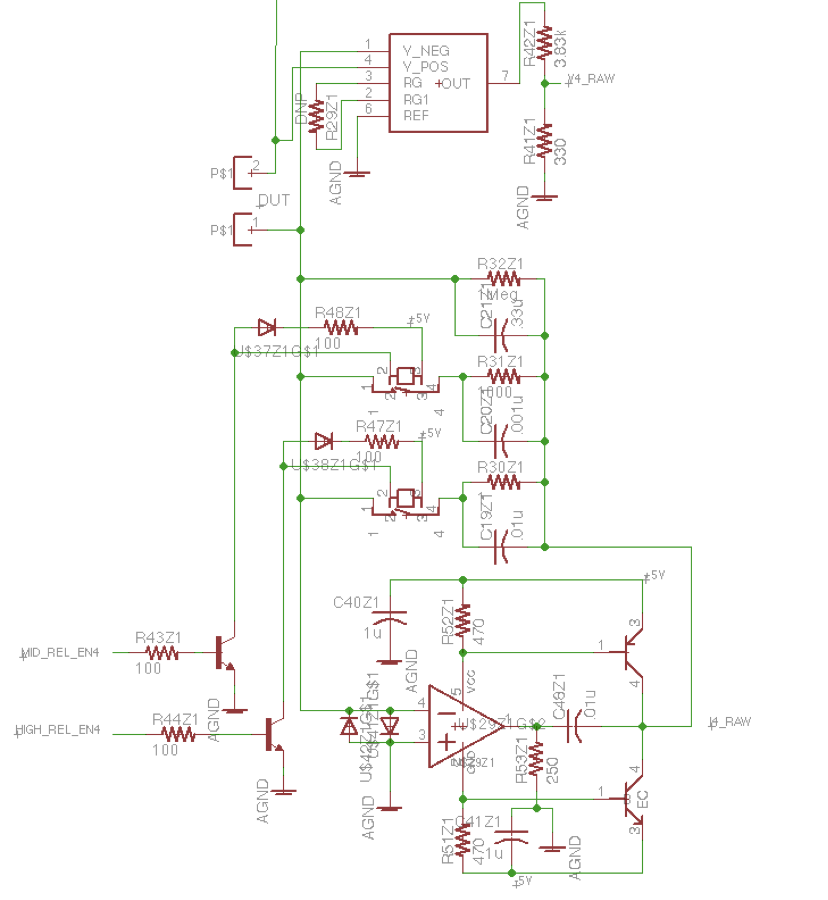
\includegraphics[width=3.5in]{measCir}
\caption{Measurement Circuitry}
\label{fig:measCir}
\end{figure}

The measurement circuitry (Fig. ~\ref{fig:measCir}) implemented consists of two different parts, voltage and current measurements. The voltage of the DUT is measured differentially by an Analog Device’s AD8220 JFET instrumentation amplifier. This output is scaled and then sent to a 12-bit DAC. The current through the DUT is measure from a low side measurement topology known and a transimpedance amplifier. The amplifier creates a virtual ground at the negative terminal of the op-amp, U39, that allows for a current reading without subjecting the measurement circuitry to a high voltage and without floating the bottom of the DUT above ground.

Since it is desirable the measure both the anodization current and the leakage current, a basic transimpedance amplifier design was modified to include three switched feedback paths. This allows the current measurement to measure currents over eight orders of magnitude. The circuitry can handle currents from 10nA to 100mA. The three current ranges are listed in Table:~\ref{tab:dacRes}.

The real measurement circuitry has several practical limitations that limit it from performing ideally. Both the differential amplifier and the transimpedance amplifier send their signals to 6-pole Sallen-Key filters. These filters have a cutoff frequency of 10kHz\cite{sThesis} in order to filter out high frequency harmonics and other undesirable noise. Any signals higher than this will be severely attenuated in the captured data.

The DACs inject digitization errors into the measurement signals. They are able to measure signals with resolutions shown in Table:~\ref{tab:dacRes}.


\begin{table}[here]
\renewcommand{\arraystretch}{1.3}
\caption{DAC Resolution}
\label{tab:dacRes}
\centering
\begin{tabular}{c|c|c}
\hline
\bfseries Resolution & \bfseries Full Scale Measurement & \bfseries Comment\\
\hline\hline
7.32mV & 30V & \\
\hline
.098mA & 100mA & Hi Current (1A-1mA)\\
\hline
.98uA & 1mA & Med Current (1mA-1uA) \\
\hline
.98nA & 1uA & Lo Current (1uA-1nA)\\
\hline
\end{tabular}
\end{table}

Once the data is collected by the microcontroller, it is sent to a PC via USB for further analysis. The data is sampled by the ADCs at a rate of baud and transferred to the PC at a rate of 2Mbaud. This allows for maximum flexibility on the PC side, where any data coming in at a rate greater than what is desired can simply be discarded.

\section{Experimental Procedure}
The experimental setup to anodize the anode of a titanium capacitor with the aforementioned circuitry is as follows. The anode sample is prepared by cleaning the surface oxide off with a chemical bath. It is then placed in a beaker of anodizing solution. The current source is connected to the DUT and acts as both a current source and data logger until the test is finished and the current through the DUT has dropped to the leakage current.

\section{Experimental Results}
Typical results from early materials can be found it Fig. 7. For additional data and complete testing curves, see \cite{sThesis} and \cite{mThesis}.


\begin{figure}[here]
\centering
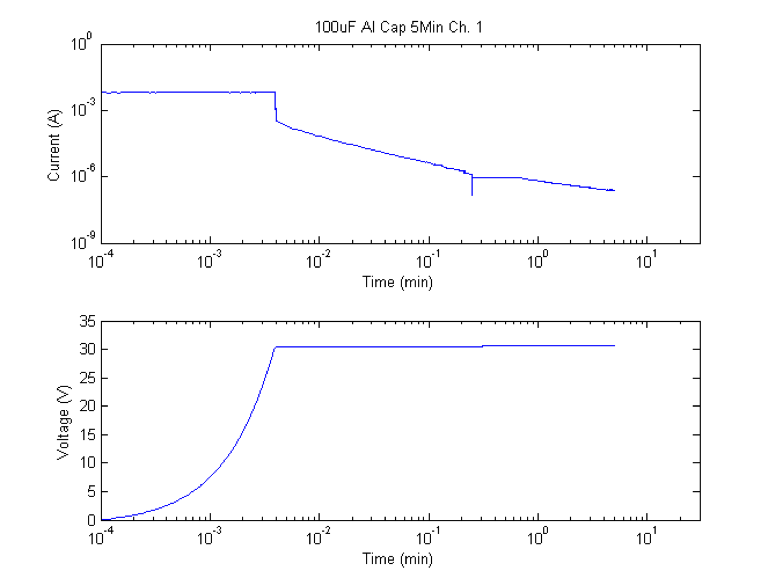
\includegraphics[width=3.5in]{measData}
\caption{Typical Results}
\label{fig:measData}
\end{figure}

% use section* for acknowledgement
\section*{Acknowledgments}

The author would like to thank...

ARPA-E,
Steven Ehret,
Dr. Francis Merat,
Dr. Gerhard Welsch,
Laurie Dudik,
and Donald McGervey

% Can use something like this to put references on a page
% by themselves when using endfloat and the captionsoff option.
\ifCLASSOPTIONcaptionsoff
\newpage
\fi

\bibliographystyle{IEEEtran}
%\bibliography{IEEEabrv,mybibfile}
\begin{thebibliography}{1}

\bibitem{tiSponge} K. Jun-Wan, \emph{"Titanium Sponge on Titanium Substrate"}, Dept. Mat. Eng., Case Western Reserve Univ., Ohio, Cleveland, 2005.

\bibitem{tiCharHag} H. Hagiwara and A. Yamashita, \emph{"H. Hagiwara and A. Yamashita, Characteristics of Titanium Electrolytic Capacitors"}, Proc. of the IEEE 1963 , pp. 1324.

\bibitem{cwruEncDie} W. Brown, D Hess, et 'all. (2006) \emph{"Dielectrics"}. [Online] Available: "http://electrochem.cwru.edu/encycl/art-a02-anodizing.htm

\bibitem{cwruEncAlanod} R. S. Alwitt. (2002, Dec.) \emph{"Anodization"}. Boundary Technologies, Inc., Northbrook, IL. [Online], Available: http://electrochem.cwru.edu/encycl/art-a02-anodizing.htm

\bibitem{tiMinit} F. Huber and J. Bloxom, \emph{"Titanium Printed Capacitors fro Mcirominiturization"}, IRE Transactions on Component Parts 1961, pp. 1-4.

\bibitem{sThesis} S. Ehret, \emph{"Instrumentation For Anodization and In-Situ Testing of Titanium Alloys For Capacitor Anodes"}, Dept. Elec. Eng., Case Western Reserve Univ., Ohio, Cleveland, 2011.

\bibitem{mThesis} M. DeLibero, \emph{"Instrumentation for the Evaluation of Titanium Electrolytic Capacitors"}, Dept. Elec. Eng., Case Western Reserve Univ., Ohio, Cleveland, Jun. 2012.

\end{thebibliography} 

\end{document}

